\section{Resultados Experimentales}

En esta sección se presenta un resumen de los resultados experimentales obtenidos utilizando el algoritmo \textit{Regret Matching} en los juegos descritos. Cada procedimiento fue probado $10$ veces por juego, finalizando cada corrida cuando se obtenía un regret máximo menor que $0.005$.

La tabla \ref{tab:resumen-resultados-RM} muestra un resumen de los resultados. En esta tabla se muestra, por cada juego, el tamaño de la matriz de pagos, el valor teórico del juego ($u_t$), el valor del juego utilizando la estrategia obtenida en la última corrida del algoritmo ($u_e$) y la explotabilidad ($\varepsilon_{\sigma}$). Las dos últimas métricas se presentan para cada uno de los procedimientos (A, B y C). En todos los casos se observa que la utilidad esperada para las estrategias obtenidas es cercana al valor del juego, además, se obtuvo una explotabilidad menor o igual que $0.011$, por lo que las estrategias obtenidas representan buenas aproximaciones al equilibrio de Nash en cada juego.

\begin{table}[htpb]
    \centering
    \begin{tabular}{l|r|r r r|r r r}
        &  & \multicolumn{3}{|c}{$u_e$} & \multicolumn{3}{|c}{$\varepsilon_{\sigma}$}  \\ \hline
        Juegos & $u_t$ & \multicolumn{1}{|c}{A} & \multicolumn{1}{c}{B} & \multicolumn{1}{c|}{C}
          & \multicolumn{1}{|c}{A} & \multicolumn{1}{c}{B} & \multicolumn{1}{c}{C} \\ \hline
        Matching Pennies
            & $0$ & $0$ & $0$ & $0$ & $0.006$ & $0.006$ & $0.008$ \\
        Piedra, Papel o Tijeras
            & $0$ & $-0.000012$ & $0.000004$ & $0.000022$ & $0.006$ & $0.01$ & $0.009$ \\
        Ficha vs. Dominó
            & $\frac{1}{3}$ & $0.333$ & $0.334$ & $0.334$ & $0.01$ & $0.007$ & $0.004$ \\
        Coronel Blotto
            & $0$ & $0.000219$ & $-0.000502$ & $0.000024$ & $0.01$ & $0.011$ & $0.009$ \\
        \hline
    \end{tabular}
    \caption{Resumen de los resultados y evaluación de las estrategias obtenidas usando el algoritmo de Regret Matching en juegos en forma normal}
    \label{tab:resumen-resultados-RM}
\end{table}

Para evaluar la convergencia se midió el tiempo necesario para alcanzar el regret desea y el número de iteraciones, en la Tabla \ref{tab:resumen-regret-tiempo-RM} se presenta el tiempo ($T$), el número de iteraciones ($I$) y el tiempo por iteración ($T/I$) obtenido para cada uno de los juegos para cada procedimiento. Estos resultados son el promedio de las $10$ corridas realizadas por juego y procedimiento. Además, se crearon gráficas del regret por iteración para observar como disminuye a medida que corre el algoritmo, la  Figura  \ref{fig:regret-blotto} muestra las gráficas para el juego Coronel Blotto y los $3$ procedimientos. Estas gráficas son mostradadas con una escala logarítmica en el eje $x$ para apreciar mejor los resultados. En el Apéndice A se muestran las tablas detalladas con los resultados en cada una de las corridas y las gráficas de cada juego con los $3$ procedimientos.

\begin{figure}[htpb!]
    \caption{Gráficas del regret con respecto al número de iteraciones del juego Coronel Blotto}
    \label{fig:regret-blotto}
    \centering
    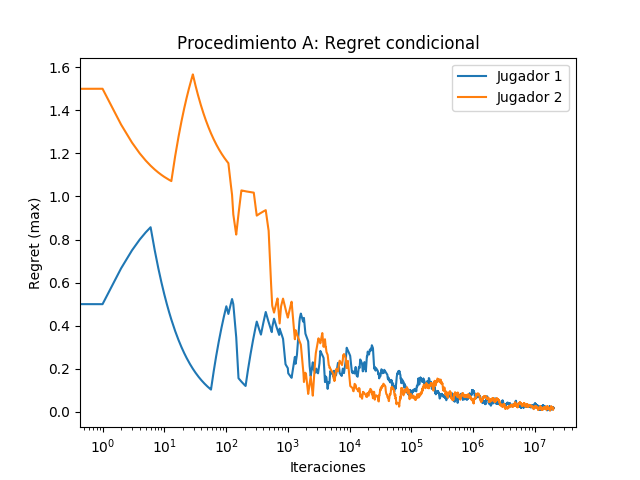
\includegraphics[width=0.58\textwidth]{graficas/coronel-blotto/procedimiento-A.png}
    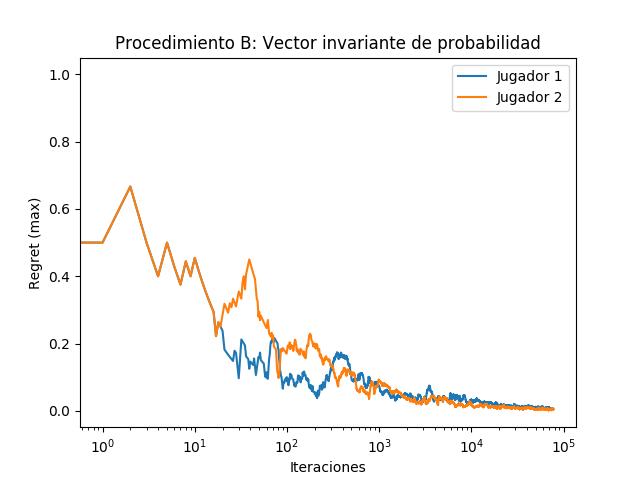
\includegraphics[width=0.58\textwidth]{graficas/coronel-blotto/procedimiento-B.png}
    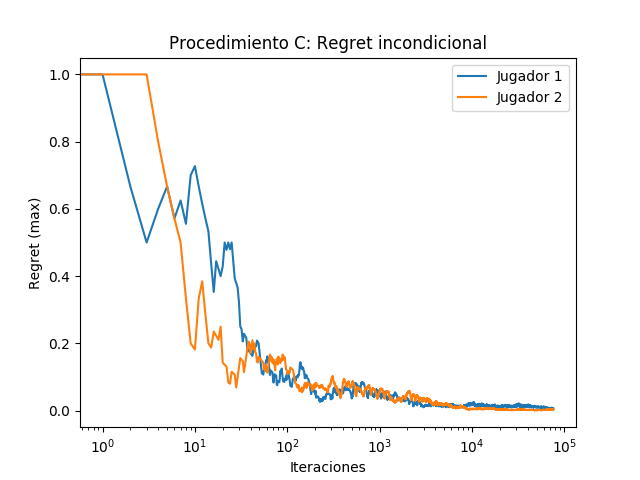
\includegraphics[width=0.58\textwidth]{graficas/coronel-blotto/procedimiento-C.png}
\end{figure}

\begin{table}[htpb]
    \centering
    \begin{tabular}{l | c |r r r}
        Juegos & Proc. & $T$ & $I$ & $T/I$ \\ \hline
        \multirow{3}{*}{Matching Pennies}
            & A & $10.276$ & $3892550.4$ & $2.64 {\times} 10^{-06}$ \\
            & B &  $0.777$ &   $25616.6$ & $3.03 {\times} 10^{-05}$ \\
            & C &  $0.042$ &   $16260.5$ & $2.58 {\times} 10^{-06}$ \\ \hline
        \multirow{3}{*}{Piedra, Papel o Tijeras}
            & A & $12.198$ & $4519054.1$ & $2.70 {\times} 10^{-06}$ \\
            & B &  $0.345$ &    $6601.3$ & $5.23 {\times} 10^{-05}$ \\
            & C &  $0.049$ &   $19321.1$ & $2.54 {\times} 10^{-06}$ \\ \hline
        \multirow{3}{*}{Ficha vs. Dominó}
            & A & $319.179$ & $108319272.4$ & $2.95 {\times} 10^{-06}$ \\
            & B &  $11.275$ &     $75250.2$ & $1.50 {\times} 10^{-04}$ \\
            & C &   $0.237$ &     $84318.5$ & $2.81 {\times} 10^{-06}$ \\ \hline
        \multirow{3}{*}{Coronel Blotto}
            & A & $875.533$ & $190222305.3$ & $4.60 {\times} 10^{-06}$ \\
            & B &  $79.358$ &     $66378.4$ & $1.20 {\times} 10^{-03}$ \\
            & C &   $0.166$ &     $48613.5$ & $3.41 {\times} 10^{-06}$ \\ \hline
    \end{tabular}
    \caption{Resumen de los resultados y evaluación de las estrategias obtenidas usando el algoritmo de Regret Matching en juegos en forma normal}
    \label{tab:resumen-regret-tiempo-RM}
\end{table}

A continuación se se analiza el desempeño de los procedimientos, comparándolos entre sí, observando la rapidez de convergencia de cada uno de ellos.

\subsection{Complejidad de cada iteración}

Los procedimientos cambian en la forma en que se elige la siguiente estrategia en cada iteración. En los procedimientos A y B se utiliza un regret condicional, en el que se mide el \textit{arrepentimiento} de cambiar una estrategia por otra en específica. Esta métrica se debe mantener a lo largo de todas las iteraciones, por lo que cada iteración necesita memoria adicional de complejidad $\mathcal{O}(N^2 + M^2)$, donde $N$ y $M$ es el número de acciones posibles para el jugador $1$ y $2$, respectivamente. En el procedimiento C se utiliza únicamente el regret incondicional, por lo que la cantidad de memoria adicional es del orden $\mathcal{O}(N + M)$.

Con respecto a la complejidad de tiempo se tiene que los procedimientos de regret condicional e incondicional (A y C), son lineales al número de acciones. Sin embargo, en el procedimiento B es necesario resolver un sistema de ecuaciones lineales para elegir cada estrategia nueva, del tamaño del número de acciones del jugador respectivo, obteniendo que la complejidad total es $\mathcal{O}(N^3 + M^3)$. La Tabla \ref{tab:complejidades-iteraciones} muestra un resumen de la complejidad es tiempo y memoria adicional.

\begin{table}[ht]
    \centering
    \begin{tabular}{c|c|c}
         Procedimiento & Memoria & Tiempo  \\ \hline
         A & $\mathcal{O}(N^2 + M^2)$ & $\mathcal{O}(N + M)$ \\ 
         B & $\mathcal{O}(N^2 + M^2)$ & $\mathcal{O}(N^3 + M^3)$ \\
         C & $\mathcal{O}(N + M)$     & $\mathcal{O}(N + M)$ \\ \hline
    \end{tabular}
    \caption{Complejidad por iteración de cada uno de los procedimientos}
    \label{tab:complejidades-iteraciones}
\end{table}

Por lo anterior, se observa que la velocidad de las iteraciones del procedimiento que calcula el vector invariante de probabilidad es más lenta en todos los casos, estando uno o dos órdenes de magnitud por encima, según el tamaño de la matriz. Por lo que, si la matriz es sumamente grande, el segundo método sería el menos adecuado.

\subsection{Número de iteraciones}

En la Tabla \ref{tab:resumen-regret-tiempo-RM} se puede observar un resumen de las iteraciones promedio de los tres procedimientos en cada uno de los juegos. Se nota que el procedimiento A, regret incondicional es el que necesita muchas más iteraciones para converger. Con respecto a los procedimientos B y C, se observa que en algunos casos el promedio en el procedimiento B fue menor y en otros el promedio del procedimiento C. También es importante destacar que en el juego de piedra, papel o tijera se tienen varios casos donde se obtiene la convergencia en menos de $10$ iteraciones (ver apéndice A), esos son casos donde se obtiene el equilibrio de Nash de forma exacta en pocas iteraciones.

\subsection{Tiempo transcurrido}

Observando el tiempo promedio de los procedimientos en la tabla \ref{tab:resumen-regret-tiempo-RM}, se nota que el procedimiento A es el que emplea más tiempo en todos los casos, esto ocurre porque necesita muchas más iteraciones que los otros dos procedimientos. Por otra parte el procedimiento C es también más rápido que el procedimiento B, ya que la complejidad en cada iteración para resolver el sistema de ecuaciones enlentece el tiempo total necesario, incluso, si la matriz es muy grande este procedimiento podría ser más lento que el procedimiento A y no sería factible.

Aunque el procedimiento donde se aplica regret matching al regret incondicional (procedimiento C), es el más sencillo de implementar y el más rápido en converger, este procedimiento tiene una desventaja con respecto a los otros dos. Al utilizar el regret condicional, los dos primeros procedimientos garantizan que el regret condicional tiende a cero para cualquier par de estrategias de cada jugador y por lo tanto, conducen siempre a un equilibrio correlacionado. El tercer procedimiento sólo minimiza el regret incondicional y por lo tanto, si el juego es de más de dos jugadores o no es de suma cero, entonces ya no es de utilidad para hallar alguna solución del juego.

